\chapter{Construction Method and Planning}

\section{Construction Method}

The main steps during construction are:
\begin{enumerate}
 \item Reposition old core
 \item Place core
 \item Place sublayer
 \item Place armour layer on landward side
 \item Place toe
 \item Place armour layer on seaward side
 \item Construct road and top structure
\end{enumerate}

\paragraph{Reposition old core}
To increase available space on the side of the harbour the old core is repositioned by moving the armour layer on the harbour side to the seaward side.
The total width of the old breakwater is about 70m at ground level, which poses restrictions on the equipment, that can be used.
Waterborne equipment is not a good choice for this task.
The rocks picked up on the one side (for instance by a hydraulic excavator/crane on a pontoon) would need to be transported to the other side (by a barge for instance), since the hydraulic excavator/ crane would not be able to reach all the way over the old breakwater.
Therefore a landbased long reach hydraulic excavator is used.
For instance Hitachi ZX850 with a reach of 27m and 2m³ bucket capacity could be used\footnote{http://www.land-water.co.uk/group-services/plant-hire-2/long-reach/zx-850-27m-long-reach-excavator/}.
According to \citet{cem} rocks with 0 to 5t have a nominal diameter of maximum 1.38m, thus an average volume of $\frac{4}{3}\Pi \cdot \left(\frac{1.38m}{2}\right)^{3}=1.4m^3<2m^3$, which is smaller than the bucket capacity.
Since the old breakwater is in general expected to be not accessible any more a temporary road will be built buy placing gravel with dump trucks and make them even with a bulldozer (starting from the landside and proceeding to tip of breakwater).
At the end a place to turn around is built.
The width is 8m at least, so two trucks can easily pass each other and a crane or hydraulic excavator at some point does not hinder the truck transport.
For parts of the old breakwater, where the damage is even more severe than depicted in cross-section A-A and B-B a hydraulic excavator/crane on a pontoon will be available to move rocks out of reach of the long reach hydraulic excavator inside its reach.

\paragraph{Place core}
The rocks for the core are delivered from quarry Kruj\"{e}.
There rocks up to 2t are available \citep{MScRomano}.
The distance of about 50km can easily be travelled by trucks (see \ref{fig:mapConstruction}). 
Class 0.3t to 1t is used.
Using the temporary road first on the slopes the needed core material is placed with dump trucks directly coming from the quarry and hydraulic excavators to construct the slope.
This can be done at several positions at one time, depending on the availability of hydraulic excavators and dump trucks.
Then starting from the tip of the breakwater the needed height of the core will be built.

\paragraph{Place sublayer}
The sublayer is made of rocks of up to 2.5t.
The maximum rocks of 2t , which are the largest rocks available via the quarry Kruj\"{e} \citep{MScRomano}.
The distance of about 50km (see \ref{fig:mapConstruction}) can easily be travelled by trucks.
The grading delivered will be divided and rocks smaller than 2t will be used to fill the rest of the core.



\begin{figure}[!htb]
  \center
  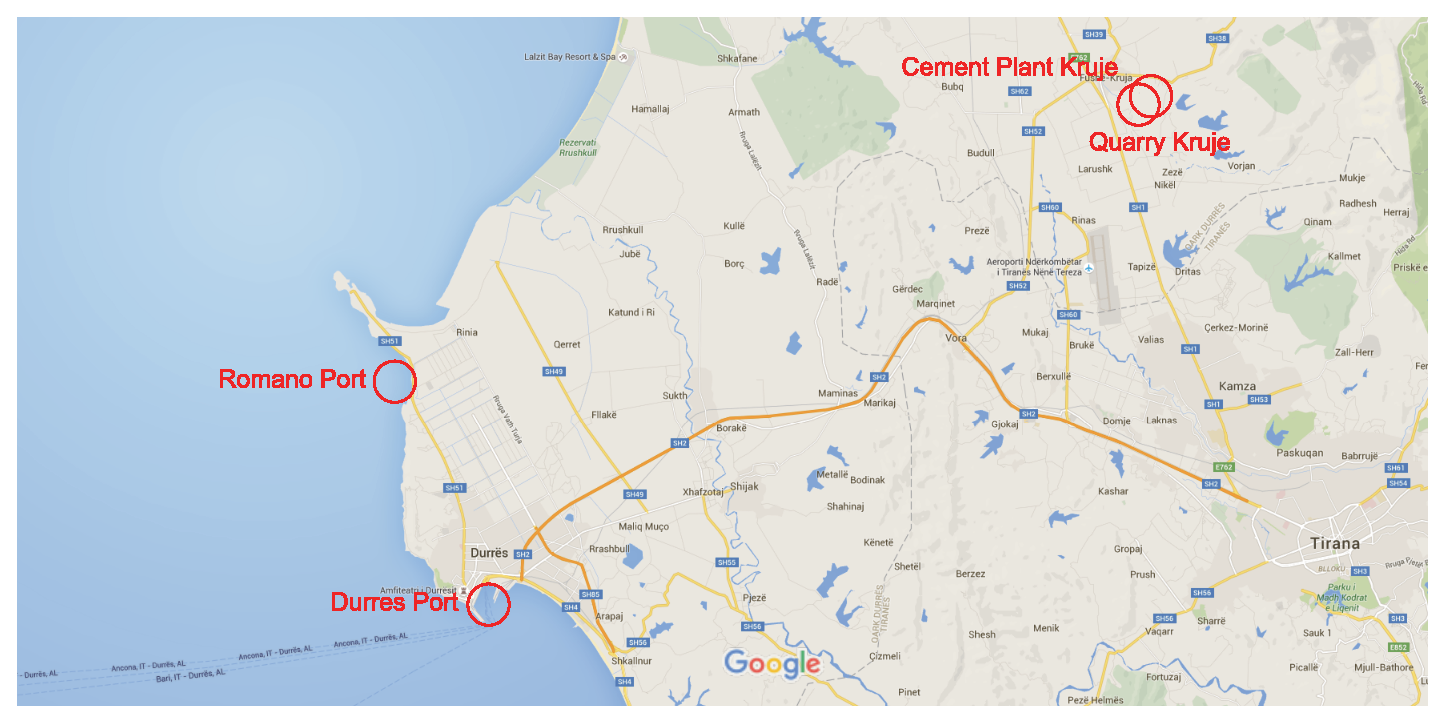
\includegraphics[width=\textwidth]{images/mapConstruction} 
  \caption{Location of facilities needed for construction (map from maps.google.com)}
  \label{fig:mapConstruction}
\end{figure}


To show how the different steps given above interlock with each other see \nameref{chap:appendixB}.

\section{Production Calculation}